\sectioncounter{34}

\section{直线与平面的垂直}

\subsection{知识梳理}

若直线 $l$ 与平面 $\alpha$ 内的任意一条直线都垂直, 则称 $l$ 与 $\alpha$ 互相垂直, 记作 $l\perp \alpha$. 此时, $l$ 叫做 $\alpha$ 的垂线, $\alpha$ 叫做 $l$ 的垂面, $l$ 与 $\alpha$ 唯一的公共点称为垂足.

线面垂直判定定理:直线与平面内两条相交直线都垂直, 则该直线与此平面垂直.

对应的符号语言 (图 \ref{fig-190702-1930}): $a$, $b\subset\alpha$, $a\cap b= P$, $l\perp a$, $l\perp b\Rightarrow l\perp \alpha$.

当直线 $l$ 与平面 $\alpha$ 垂直时, 由定义知, $l$ 与 $\alpha$ 内任意直线垂直. 当直线 $a$,$b$ 均与平面 $\alpha$ 垂直时, 可得 $a\parallel b$.

线面垂直性质定理:垂直于同一个平面的两条直线平行.

对应的符号语言 (图 \ref{fig-190702-1940}): $a\perp\alpha$, $b\perp\alpha\Rightarrow a\parallel b$.

    \begin{figure}[htb]
    \small
    \centering
    \begin{minipage}[b]{0.45\linewidth}
      \centering
      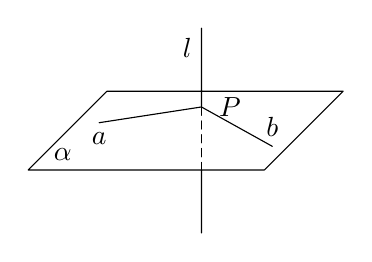
\begin{tikzpicture}[line cap=round,line join=round,scale=1]
        \draw (0,0) coordinate (A) +(0.2,0) node[anchor=south west] {$\alpha$}
          (3,0) coordinate (B) (1,1) coordinate (D)
          (B)++(D) coordinate (C) 
          (0.9,0.6) coordinate (a) node[below] {$a$}
          (2.2,0.8) coordinate (P) +(0.1,0) node[right] {$P$}
          (3.1,0.3) coordinate (b) node[above] {$b$}
          (2.2,-0.8) coordinate (l1) (2.2,0) coordinate (l2)
          (2.2,1.8) coordinate (l3) node[anchor= north east] {$l$};
        
        \draw (A)--(B)--(C)--(D)--(A) (l1)--(l2) (P)--(l3) (a)--(P)--(b);
        \draw[densely dashed] (P)--(l2);
      \end{tikzpicture}
      \caption{}\label{fig-190702-1930}
    \end{minipage}
    \hskip 0.5cm  
    \begin{minipage}[b]{0.45\linewidth}
      \centering
      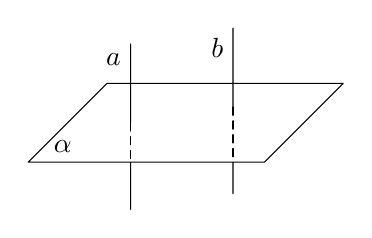
\begin{tikzpicture}[line cap=round,line join=round,scale=1]
        \def\ax{1.3} \def\bx{2.6}
        \draw (0,0) coordinate (A) +(0.2,0) node[anchor=south west] {$\alpha$}
          (3,0) coordinate (B) (1,1) coordinate (D)
          (B)++(D) coordinate (C)
          (\ax,1.5) coordinate (a1) node[anchor= north east] {$a$}
          (\ax,0.5) coordinate (a2) (\ax,0) coordinate (a3) 
          (\ax,-0.6) coordinate (a4) 
          (\bx,1.7) coordinate (b1) node[anchor= north east] {$b$}
          (\bx,0.7) coordinate (b2) (\bx,0) coordinate (b3) 
          (\bx,-0.4) coordinate (b4) ;
        
        \draw (A)--(B)--(C)--(D)--(A) (a1)--(a2) (a3)--(a4) (b1)--(b2) (b3)--(b4);
        \draw[densely dashed] (a2)--(a3) (b2)--(b3);
      \end{tikzpicture}
      \caption{}\label{fig-190702-1940}
    \end{minipage}
    \end{figure}

直线 $PA$ 与平面 $\alpha$ 交于点 $A$, 且 $PA$ 不与 $\alpha$ 垂直, 则称 $PA$ 为 $\alpha$ 的斜线, 点 $A$ 为斜足 (图 \ref{fig-211107-1525}). 过点 $P$ 作 $PO\perp\alpha$, 则直线 $AO$ 称为 $PA$ 在 $\alpha$ 上的射影 (或投影), $\angle PAO$ 称为 $PA$ 与 $\alpha$ 所成的角 (必为锐角). 若直线与平面垂直, 则称它们所成的角为直角; 若线面平行或线在面内, 则称它们所成的角为零角.

\begin{figure}[htb]
  \small\centering
  \includegraphics[scale=1.4]{2021-1107-1525-crop}
  \caption{}\label{fig-211107-1525}
\end{figure}

\lianxi

\begin{exercise}
    若直线 $a$ 上有两点到平面 $\alpha$ 的距离相等, 判断 $a$ 与 $\alpha$ 
    的位置关系.
\end{exercise}
\beginsolution
    平行或相交. 对后一情形, 题中两点在交点异侧.
\endsolution

\begin{exercise}
    平面 $\alpha$,$\beta$,$\alpha_1$,$\beta_1$ 满足 $\alpha\perp \alpha_1$, $\beta\perp\beta_1$, $\alpha\perp \beta$, 判断 $\alpha_1$,$\beta_1$ 的位置关系.
\end{exercise}
\beginsolution
    $\alpha_1$,$\beta_1$ 可能平行 (含重合) 或相交.
\endsolution

\begin{exercise}
    如图 \ref{fig-190702-1950} 所示, 在四棱锥 $P\text{--}ABCD$ 中, 四边形 $ABCD$ 是正方形, $PA\perp$ 平面 $ABCD$, $PA=AB$, 求:
    
    (1) $PC$ 与平面 $ABCD$ 所成角的正切值;
    
    (2) $PB$ 与平面 $PAC$ 所成角的大小.
\end{exercise}
\beginsolution
    (1) 因为 $PA\perp$ 平面 $ABCD$, 所以 $PA\perp AC$, $PC$ 与平面 $ABCD$ 所成角为 $\angle PCA$. 设 $PA=AB=a$, 则在正方形 $ABCD$ 中, $AC=\sqrt2 a$, 所以
    \[\tan\angle PCA= \frac{PA}{PC}= \frac{a}{\sqrt2 a}
        = \frac{\sqrt2}{2}.\]

    (2) 连接 $BD$ 并设 $BD$ 与 $AC$ 交于点 $O$, 再连接 $PO$, 则在正方形 $ABCD$ 中, $BD\perp AC$. 由 $PA\perp$ 平面 $ABCD$ 知, $PA\perp BD$, 所以 $BD\perp$ 平面  $PAC$, 则 $BO\perp PO$, $PB$ 与平面 $PAC$ 所成的角为 $\angle BPD$. 
    \mymarginpar{求 $\angle BPO$ 的大小也可利用
    \[PB= BD= PD= \sqrt2 a.\]}
    因为 $BO= \dfrac12 BD= \dfrac{\sqrt2}2 a$,
    \[PO= \sqrt{PA^2+ AO^2}= \sqrt{a^2+\frac{a^2}2}
        = \frac{\sqrt6}2 a,\]
    所以 
    \[\tan\angle BPO= \frac{BO}{PO}= \frac{1}{\sqrt3}
        = \frac{\sqrt3}{3},\]
    从而 $\angle BPO= 30^\circ$.
\endsolution

    \begin{figure}[htb]
    \small
    \centering
    \begin{minipage}[b]{0.45\linewidth}
      \centering
      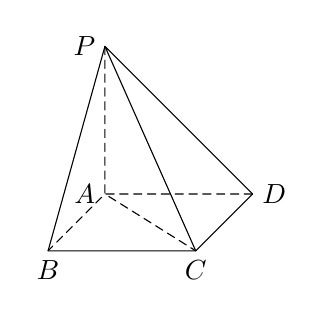
\begin{tikzpicture}[line cap=round,line join=round,scale=0.75]
        \def\AB{2.5}        
        \draw (0,0,0) coordinate (A) node[left] {$A$}
          (0,0,\AB) coordinate (B) node[below] {$B$}
          (\AB,0,0) coordinate (D) node[right] {$D$}
          (B)++(D) coordinate (C) node[below] {$C$}
          (A)++(0,\AB,0) coordinate (P) node[left] {$P$};
        
        \draw (P)--(B)--(C)--(D)--(P)--(C);
        \draw[densely dashed] (P)--(A)--(B) (D)--(A)--(C);      
      \end{tikzpicture}
      \caption{}\label{fig-190702-1950}
    \end{minipage}
    \hskip 0.5cm  
    \begin{minipage}[b]{0.45\linewidth}
      \centering
      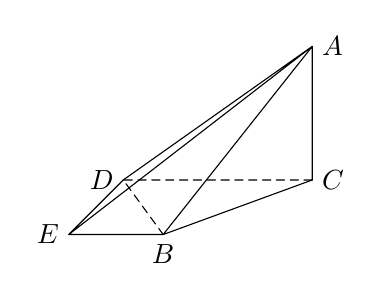
\begin{tikzpicture}[line cap=round,line join=round,scale=1.2]
        \draw (2,1.414,0) coordinate (A) node[right] {$A$}
          (1,0,1.5) coordinate (B) node[below] {$B$}
          (2,0,0) coordinate (C) node[right] {$C$}
          (0,0,0) coordinate (D) node[left] {$D$}
          (0,0,1.5) coordinate (E) node[left] {$E$};
        
        \draw (E)--(D)--(A)--(E)--(B)--(C)--(A)--(B);
        \draw[densely dashed] (C)--(D)--(B);
      \end{tikzpicture}
      \caption{}\label{fig-190702-2000}
    \end{minipage}
    \end{figure}

\subsection{要点导学\quad 各个击破}
\subsubsection{直线与平面垂直的判定}
\begin{example}
    如图 \ref{fig-190702-2000} 所示, 在四棱锥 $A\text{--}BCDE$ 中, $AC\perp DC$, $\angle CDE=\angle BED=90^\circ$, $AB=CD=2$, $DE=BE=1$, $AC=\sqrt2$. 求证: $DE\perp$ 平面 $ACD$.
\end{example}
\beginsolution
    过点 $B$ 作 $BF\perp CD$ 于 $F$, 则四边形 $BEDF$ 为矩形,
    \[BF= DE= 1,\quad DF= EB= 1.\]
    因为 $CD=2$, 所以 $CF=1$, $CB=\sqrt2$. 而 $AB=2$, $AC=\sqrt2$, 所以
    \[AB^2= BC^2+AC^2,\quad\text{即}\quad
        AC\perp BC.\]
    由 $AC\perp DC$ 知 $AC\perp$ 平面 $BCD$, 所以 $AC\perp DE$. 因为 $\angle CDE=90^\circ$, 所以 $DE\perp CD$, 故 $DE\perp$ 平面 $ACD$.
\endsolution

\lianxi
\begin{exercise}[s]
    如图 \ref{fig-190702-2010} 所示, $AB$ 是圆 $O$ 的直径, $PA$ 垂直于圆 $O$ 所在的平面, $C$ 是圆 $O$ 上异于 $A$,$B$ 的点. 求证: $BC\perp$ 平面 $PAC$.
\end{exercise}
\beginsolution
    因为 $AB$ 是直径, 所以 $\angle ACB= 90^\circ$, $AC\perp CB$. 又因为 $PA\perp$ 平面 $ACB$, 所以 $PA\perp BC$, 则 $BC\perp$ 平面 $PAC$.
\endsolution

    \begin{figure}[htb]
    \small
    \centering
    \begin{minipage}[b]{0.45\linewidth}
      \centering
      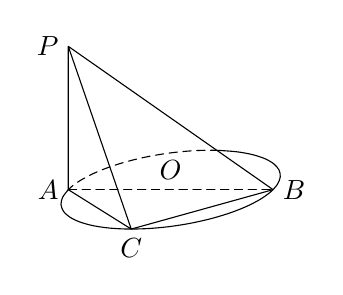
\begin{tikzpicture}[line cap=round,line join=round,scale=1.3]        
        \draw (0,0,0) coordinate (O) node[above] {$O$}
          (-1,0,0) coordinate (A) node[left] {$A$}
          (1,0,0) coordinate (B) node[right] {$B$}
          (0,0,1) coordinate (C) node[below] {$C$}
          (A)++(0,1.4,0) coordinate (P) node[left] {$P$};
        \draw[domain=-90:175,smooth,variable=\t] 
          plot ({sin(\t)},0,{cos(\t)});
        \draw[domain=175:270,smooth,variable=\t,densely dashed] 
          plot ({sin(\t)},0,{cos(\t)});
        
        \draw (P)--(B)--(C)--(A)--(P)--(C);
        \draw[densely dashed] (A)--(B);      
      \end{tikzpicture}
      \caption{}\label{fig-190702-2010}
    \end{minipage}
    \hskip 0.5cm  
    \begin{minipage}[b]{0.45\linewidth}
      \centering
      \begin{tikzpicture}[line cap=round,line join=round,scale=1.4]
        \draw (-0.15,0,1.414) coordinate (A) node[below] {$A$}
          (1,0,0) coordinate (C) node[right] {$C$}
          (A)++(C) coordinate (B) node[below] {$B$}
          (0,0,0) coordinate (D) node[left] {$D$}
          ($(D)!0.5!(C)$) coordinate (O) node[below] {$O$}
          (0.5,1.2,0) coordinate (E) node[left] {$E$}
          ($(B)!0.5!(C)$) coordinate (F) node[right] {$F$};
        
        \draw (E)--(A)--(B)--(E)--(C)--(B) (E)--(F);
        \draw[densely dashed] (C)--(D)--(E)--(O) (D)--(A)--(F);
      \end{tikzpicture}
      \caption{}\label{fig-190702-2020}
    \end{minipage}
    \end{figure}
    
\subsubsection{直线与平面垂直的性质}
\begin{example}
    如图 \ref{fig-190702-2020} 所示, 四棱锥 $E\text{--}ABCD$ 中, 四边形 $ABCD$ 是矩形, $BC=\sqrt2 AB$, $O$,$F$ 分别为 $CD$,$BC$ 的中点, $EO\perp$ 平面 $ABCD$, 求证: $AF\perp EF$.
\end{example}
\beginsolution
    连接 $OF$. 设 $AB=2a$, 则 $BC= 2\sqrt2 a$. 由 $O$,$F$ 分别为 $CD$,$BC$ 的中点知,
    \[BF= FC= \sqrt2 a,\quad OC= a.\]
    因为四边形 $ABCD$ 是矩形, 
    \mymarginpar{本题中矩形 $ABCD$ 的邻边长度比为 $\sqrt2$, 是特殊的比值, 也可利用相似证明 $AF\perp FO$, 且证法与题中三角函数证法等价.}
    所以 $\angle ABF= \angle FCO= 90^\circ$, 且
    \[\tan\angle AFB= \frac{AB}{BF}= \sqrt2,\quad
    \tan\angle FOC= \frac{FC}{CO}= \sqrt2,\]
    即 $\angle AFB= \angle FOC$. 因此
    \[\angle AFB+\angle CFO= \angle FOC+\angle CFO= 90^\circ,\]
    表明 $\angle AFO= 90^\circ$, 即 $AF\perp FO$. 因为 $EO\perp$ 平面 $ABCD$, 所以 $EO\perp AF$, 则 $AF\perp$ 平面 $EOF$, 从而 $AF\perp EF$.
\endsolution

\lianxi
\begin{exercise}
    如图 \ref{fig-190702-2210} 所示, 在四棱锥 $P\text{--}ABCD$ 中, 底面 $ABCD$ 为平行四边形, $\angle DAB=60^\circ$, $AB=2AD$, $PD\perp\text{底面\ }ABCD$. 求证: $PA\perp BD$.
\end{exercise}
\beginsolution
    过点 $B$ 作 $BD'\perp AD$ 于 $D'$. 因为 $\angle DAB= 60^\circ$, 所以 $AB= 2AD'$. 由已知, $AB= 2AD$, 则 $AD=AD'$, 即点 $D$ 与 $D'$ 重合, 表明 $BD\perp AD$. 因为 $PD\perp$ 底面 $ABCD$, 所以 $PD\perp BD$, 则 $BD\perp$ 平面 $PAD$, 故 $PA\perp BD$.
\endsolution

    \begin{figure}[htb]
    \small
    \centering
    \begin{minipage}[b]{0.45\linewidth}
      \centering
      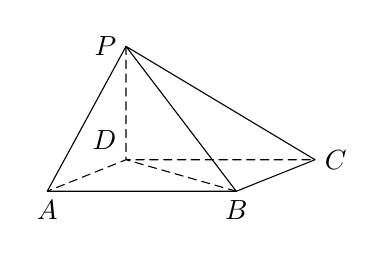
\begin{tikzpicture}[line cap=round,line join=round,scale=0.6]        
        \draw (0,0,0) coordinate (D) node[anchor=south east] {$D$}
          (-1,0,1.732) coordinate (A) node[below] {$A$}
          (4,0,0) coordinate (C) node[right] {$C$}
          (A)++(C) coordinate (B) node[below] {$B$}
          (D)++(0,2.4,0) coordinate (P) node[left] {$P$};
        
        \draw (P)--(A)--(B)--(P)--(C)--(B);
        \draw[densely dashed] (P)--(D)--(A) (B)--(D)--(C);      
      \end{tikzpicture}
      \caption{}\label{fig-190702-2210}
    \end{minipage}
    \hskip 0.5cm  
    \begin{minipage}[b]{0.45\linewidth}
      \centering
      \begin{tikzpicture}[line cap=round,line join=round,scale=0.9]
        \draw (0,0,0) coordinate (A) +(0,0.1,-0,2)node[left] {$A$}
          (0,0,2.5) coordinate (B) node[below] {$B$}
          (3,0,0) coordinate (D) node[right] {$D$}
          (B)++(D) coordinate (C) node[below] {$C$}
          (A)++(0,1.4,0) coordinate (P) node[left] {$P$}
          ($(B)!0.5!(A)$) coordinate (M) +(0.3,0,0.3) node {$M$}
          ($(P)!0.5!(C)$) coordinate (N) +(0,0,0.2) node[anchor=south west] {$N$};
        
        \draw (P)--(B)--(C)--(P)--(D)--(C);
        \draw[densely dashed] (M)--(N) (P)--(A)--(B) (D)--(A);
      \end{tikzpicture}
      \caption{}\label{fig-190702-2220}
    \end{minipage}
    \end{figure}
    
\begin{exercise}
    如图 \ref{fig-190702-2220} 所示, 在四棱锥 $P\text{--}ABCD$ 中, 底面 $ABCD$ 为矩形, $PA\perp$ 底面 $ABCD$, $M$,$N$ 分别是 $AB$,$PC$ 的中点. 求证: $MN\perp AB$.
\end{exercise}
\beginsolution
    方法一: 取 $PB$ 中点 $E$, 连接 $EM$,$EN$. 因为 $M$,$N$ 分别是 $AB$,$PC$ 的中点, 所以 $EM\parallel PA$, $EN\parallel BC$. 在矩形 $ABCD$ 中, $AB\perp BC$, 则 $AB\perp EN$. 由 $PA\perp$ 底面 $ABCD$ 知, $PA\perp AB$, 则 $EM\perp AB$, 所以 $AB\perp$ 平面 $EMN$, 故 $MN\perp AB$.

    方法二: 也可用空间向量法证明此题. 以点 $A$ 为坐标原点, $AB$,$AD$,$AP$ 分别为 $x$ 轴, $y$ 轴, $z$ 轴. 设 $B(b,0,0)$, $D(0,d,0)$, $P(0,0,p)$, 则
    \[M\Bigl(\frac{b}2,0,0\Bigr),\quad C(b,d,0),\quad
    N\Bigl(\frac{b}2,\frac{d}2,\frac{p}2\Bigr),\]
    所以 
    \[\overrightarrow{AB}= (b,0,0),\quad
        \overrightarrow{MN}= \Bigl(0,\frac{d}2,\frac{p}2\Bigr).\]
    显然 $\overrightarrow{AB}\cdot \overrightarrow{MN}=0$, 即 $MN\perp AB$.
\endsolution

\subsubsection{直线与平面垂直的探索问题}
\begin{example}
    如图 \ref{fig-190703-1810} 所示, 在四棱锥 $P\text{--}ABCD$ 中, 底面 $ABCD$ 是矩形, $PD\perp$ 平面 $ABCD$, 且 $PD=DC$. 在线段 $PB$ 上确定一点 $Q$, 使 $PC\perp$ 平面 $ADQ$, 并给出证明.
\end{example}
\beginsolution
    当 $Q$ 为 $PB$ 中点时, $PC\perp$ 平面 $ADQ$. 证明如下:

        \mymarginpar{证明的关键是确保 $EQ\parallel AD$ 和 $DE\perp PC$: 前者保证平面 $ADQ$ 就是平面 $ADEQ$, 后者保证 $PC\perp$ 平面 $ADEQ$. 若 $PD\neq DC$, 则仍可先作 $DE\perp PC$ 于 $E$, 再在平面 $PBC$ 内作 $EQ\parallel BC$ 交 $PB$ 于 $Q$, 所得的点 $Q$ 即为所求.}    
    取 $PC$ 中点 $E$, 连接 $ED$,$EQ$, 则 $EQ\parallel BC$. 因为底面 $ABCD$ 是矩形, 所以 $BC\parallel AD$, 则 $EQ\parallel AD$, 表明平面 $ADQ$ 就是平面 $ADEQ$.

    由 $PD\perp$ 平面 $ABCD$ 知 $PD\perp AD$, 而 $AD\perp DC$, 则 $AD\perp$ 平面 $PDC$, 所以 $AD\perp PC$. 因为 $AD=DC$, $E$ 为 $PC$ 中点, 所以 $ED\perp PC$, 故 $PC\perp$ 平面 $ADEQ$, 即 $PC\perp$ 平面 $ADQ$.
\endsolution

    \begin{figure}[htb]
    \small
    \centering
    \begin{minipage}[b]{0.45\linewidth}
      \centering
      \begin{tikzpicture}[line cap=round,line join=round,scale=1]        
        \draw (0,0,0) coordinate (D) +(0.1,0.05,0)node[left] {$D$}
          (0.3,0,2) coordinate (A) node[below] {$A$}
          (2,0,0) coordinate (C) node[right] {$C$}
          (A)++(C) coordinate (B) node[below] {$B$}
          (D)++(0,2,0) coordinate (P) node[left] {$P$}
          ($(B)!0.5!(P)$) coordinate (Q) node[right] {$Q$};
        
        \draw (P)--(A)--(B)--(P)--(C)--(B) (A)--(Q);
        \draw[densely dashed] (P)--(D)--(A) (Q)--(D)--(C);      
      \end{tikzpicture}
      \caption{}\label{fig-190703-1810}
    \end{minipage}
    \hskip 0.5cm  
    \begin{minipage}[b]{0.45\linewidth}
      \centering
      \begin{tikzpicture}[line cap=round,line join=round,scale=1.2]
        \draw (0,0,0) coordinate (O) +(-0.1,0,-0.1) node[below] {$O$}
          (-1.2,0,0) coordinate (A) node[left] {$A$}
          (1,0,1.3) coordinate (B) node[below] {$B$}
          ($(O)-(A)$) coordinate (C) node[right] {$C$}
          ($(O)-(B)$) coordinate (D) +(0,0,-0.1) node[left] {$D$}
          (O)++(0,1.9,0) coordinate (P) node[left] {$P$};
        
        \draw (P)--(A)--(B)--(C)--(P)--(B);
        \draw[densely dashed] (B)--(D)--(A)--(C)--(D)--(P)--(O);
      \end{tikzpicture}
      \caption{}\label{fig-190703-1820}
    \end{minipage}
    \end{figure}
    
\subsubsection{课堂评价}
\begin{exercise}
    如图 \ref{fig-190703-1820} 所示, 在四棱锥 $P\text{--}ABCD$ 中, 四边形 $ABCD$ 是平行四边形, $AC\cap BD=O$, $PA=PC$, $PB=PD$, 求证: $PO\perp$ 底面 $ABCD$.
\end{exercise}
\beginsolution
    在平行四边形 $ABCD$ 中, 点 $O$ 为 $AC$ 与 $BD$ 的中点. 结合 $PA=PC$, $PB=PD$ 知 $PO\perp AC$ 且 $PO\perp BD$, 故 $PO\perp$ 底面 $ABCD$.
\endsolution

\begin{exercise}
    如图 \ref{fig-190703-1830} 所示, 在四棱锥 $A\text{--}BCDE$ 中, 底面 $BCDE$ 是等腰梯形, $BC\parallel DE$, $\angle DCB=45^\circ$, $O$ 是 $BC$ 的中点, $AO=\sqrt3$, 且 $BC=6$, $AD=AE=2CD=2\sqrt2$. 求证: $AO\perp$ 平面 $BCD$.
\end{exercise}
\beginsolution
    连接 $OD$, $OE$. 因为 $BC=6$, $O$ 是 $BC$ 的中点, 所以 $CO=3$. 又因为 $\angle DCB= 45^\circ$, $CD=\sqrt2$, 所以在 $\triangle CDO$ 中,
    \[OD^2= CD^2+CO^2- 2CD\cdot CO\cdot \cos45^\circ
        = \sqrt5,\]
    则在 $\triangle ADO$ 中,
    \[AD^2= 8= AO^2+ DO^2,\]
    表明 $\angle AOD= 90^\circ$, 即 $AO\perp OD$. 同理可证 $AO\perp OE$, 故 $AO\perp$ 平面 $BCD$.
\endsolution

    \begin{figure}[htb]
    \small
    \centering
    \begin{minipage}[b]{0.45\linewidth}
      \centering
      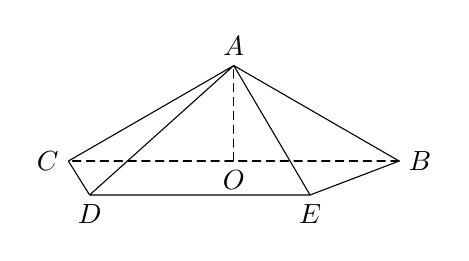
\begin{tikzpicture}[line cap=round,line join=round,scale=0.7]        
        \draw (0,0,0) coordinate (O) node[below] {$O$}
          (O)++(0,1.732,0) coordinate (A) node[above] {$A$}
          (3,0,0) coordinate (B) node[right] {$B$}
          (-3,0,0) coordinate (C) node[left] {$C$}
          (-2,0,1.6) coordinate (D) node[below] {$D$}
          (2,0,1.6) coordinate (E) node[below] {$E$};
        
        \draw (D)--(C)--(A)--(D)--(E)--(A)--(B)--(E);
        \draw[densely dashed] (O)--(A) (B)--(C);      
      \end{tikzpicture}
      \caption{}\label{fig-190703-1830}
    \end{minipage}
    \hskip 0.5cm  
    \begin{minipage}[b]{0.45\linewidth}
      \centering
      \begin{tikzpicture}[line cap=round,line join=round,scale=1.1]
        \draw (0,0,0) coordinate (O)
          (-1.5,0,0.866) coordinate (A) node[below] {$A$}
          (0.5,0,0.866) coordinate (B) node[below] {$B$}
          ($(O)-(A)$) coordinate (C) node[right] {$C$}
          ($(O)-(B)$) coordinate (D) +(0,0.1,-0.1) node[left] {$D$}
          (O)++(0,1.732,0) coordinate (P) node[left] {$P$}
          ($(P)!0.5!(A)$) coordinate (E) node[left] {$E$};
        
        \draw (P)--(A)--(B)--(C)--(P)--(B)--(E);
        \draw[densely dashed] (B)--(D)--(A) (P)--(D)--(C)--(E);
      \end{tikzpicture}
      \caption{}\label{fig-190703-1840}
    \end{minipage}
    \end{figure}

\subsection{课后练习}
\begin{exercise}
    设直线 $l$ 与平面 $\alpha$ 所成角大小为 $72^\circ$, 求 $l$ 与 $\alpha$ 内任意直线所成角大小范围.
\end{exercise}
\beginsolution
    $[72^\circ,90^\circ]$. 可以证明: 直线与平面所成的角是直线与平面内任意直线所成角的最小值.
\endsolution

\begin{exercise}
    已知四边形 $ABCD$ 为梯形, $AB\parallel CD$, $l$ 为空间一直线, 条件 $p$: $l$ 垂直于两腰 $AD, BC$, 条件 $q$: $l$ 垂直于两底 $AB, DC$, 判断 $p$ 与 $q$ 的关系 (充分性, 必要性).
\end{exercise}
\beginsolution
    充分不必要. 因为 $AB\parallel CD$, 所以 $l\perp AB$ 等价于 $l\perp DC$, 即条件 $q$ 等价于 $l$ 垂直于平面 $ABCD$ 内的一条直线.
\endsolution

\begin{exercise}
    已知直线 $l\perp$ 平面 $\alpha$, 直线 $m\subset$ 平面 $\beta$, 判断下列命题的正误:
    
    (1) $l\perp m\Rightarrow \alpha\parallel \beta$;\qquad 
    (2) $l\parallel m\Rightarrow \alpha\perp\beta$;
    
    (3) $\alpha\parallel \beta\Rightarrow l\parallel m$;\qquad
    (4) $\alpha\parallel \beta\Rightarrow l\perp m$.
\end{exercise}
\beginsolution
    (1) 错误, 由 $l\perp m$ 不能得到 $l\perp \beta$;

    (2) 正确, 由 $l\parallel m$ 知 $m\perp$ 平面 $\alpha$;

    (3) 错误, 由 $\alpha\parallel \beta$ 知 $l\perp \beta$;

    (4) 正确, 理由同上.
\endsolution

\begin{exercise}
    如图 \ref{fig-190703-1840} 所示, 四棱锥 $P\text{--}ABCD$ 的底面 $ABCD$ 是边长为 $2$ 的菱形, $\angle BAD= 60^\circ$, 且 $PB=PD=2$, $PA=\sqrt6$.
    
    (1) 求证: $PC\perp BD$;
    
    (2) 若 $E$ 为 $PA$ 的中点, 求三棱锥 $P\text{--}BCE$ 的体积.
\end{exercise}
\beginsolution
    (1) 连接 $AC$, 设其与 $BD$ 交于点 $O$, 再连接 $PO$. 因为底面 $ABCD$ 是菱形, 所以 $AC$,$BD$ 互相垂直平分于点 $O$. 由 $PB=PD$ 知 $PO\perp BD$, 所以 $BD\perp$ 平面 $PAC$, 故 $PC\perp BD$.

    (2) 因为菱形 $ABCD$ 的边长为 $2$, $\angle BAD= 60^\circ$, 所以 $\triangle ABD$ 为等边三角形, $BD=2$ 且 $AD=\sqrt3$. 结合 $PB=PD=2$ 知, $\triangle PBD$ 为等边三角形, $PO=\sqrt3$. 因为 $PA=\sqrt6$, 所以
    \[PA^2= 6= PO^2+OA^2,\]
    则 $\angle AOP= 90^\circ$, $AO\perp PO$. 而 $PO\perp BD$, 则 $PO\perp$ 底面 $ABCD$, 表明 $PO$ 为四棱锥 $P\text{--}ABCD$ 的高. 因为 $E$ 为 $PA$ 中点, 所以三棱锥 $P\text{--}BCE$ 的体积
    \[\begin{aligned}
        V_{P\text{--}BCE}
        &= \frac12 V_{P\text{--}ABC}
         = \frac14 V_{P\text{--}ABCD}\\
        &= \frac14 S_{ABCD}\cdot PO
         = \frac14\cdot 2^2 \sin 60^\circ\cdot \sqrt3\\
        &= \frac32.
    \end{aligned}\]
\endsolution

    \begin{figure}[htb]
    \small
    \centering
      \begin{tikzpicture}[line cap=round,line join=round,scale=1]
        \draw (0,0,0) coordinate (B1) node[left] {$B_1$}
          (2,0,0) coordinate (B) +(-0.1,0.1,0) node[right] {$B$}
          (B1)++(0,2,0) coordinate (A1) node[left] {$A_1$}
          (B)++(A1) coordinate (A) node[right] {$A$}
          (1.5,0,2.2) coordinate (C1) node[below] {$C_1$}
          (C1)++(B) coordinate (C) node[right] {$C$}
          ($(B)!0.5!(A)$) coordinate (G) node[left] {$G$}
          ($(C1)!0.5!(C)$) coordinate (M) node[below] {$M$}
          ($(B1)!0.5!(C)$) coordinate (N) +(-0.1,0,0) node[above] {$N$};
        
        \draw (C1)--(A1)--(B1)--(C1)--(C)--(A)--(A1) (A)--(M);
        \draw[densely dashed] (M)--(B1)--(A)--(B)--(B1)--(C)-- (B)--(N)--(G)--(C);
      \end{tikzpicture}
      \caption{}\label{fig-190703-1920}
    \end{figure}
    
\begin{exercise}
    如图 \ref{fig-190703-1920} 所示, 在直三棱柱 $ABC\text{--}A_1 B_1 C_1$ 中, $BC=CC_1$, $AB\perp BC$, $M$,$N$ 分别是 $CC_1$,$B_1C$ 的中点, $G$ 是棱 $AB$ 上的动点.
    
    (1) 求证: $B_1 C\perp$ 平面 $BNG$;
    
    (2) 试确定点 $G$ 的位置, 使 $CG\parallel$ 平面 $AB_1 M$, 并给出证明.
\end{exercise}
\beginsolution
    (1) 在直三棱柱 $ABC\text{--}A_1 B_1 C_1$ 中, $B_1B\perp$ 底面 $ABC$, 所以 $B_1B\perp AB$. 而 $AB\perp BC$, 所以 $AB\perp$ 平面 $BCC_1B_1$. 由 $BC= CC_1$ 知 $BC= BB_1$, 结合 $N$ 为 $B_1C$ 的中点知 $BN\perp B_1C$, 所以 $B_1 C\perp$ 平面 $BNG$.

    (2) 当 $G$ 为 $AB$ 的中点时, $CG\parallel$ 平面 $AB_1 M$, 证明如下:

    \mymarginpar{(2) 中线面平行的关键是存在平行四边形 $MCGH$, 故若 $M$ 不为 $C_1C$ 的中点, 则只需保证
    \[\frac{CM}{CC_1}= \frac{AG}{AB}.\]}
    取 $AB_1$ 的中点 $H$, 连接 $HG$,$HM$, 则由 $M$ 为 $CC_1$ 中点知,
    \[HG\parallel B_1B\parallel MV,\quad
        HG= \frac12 B_1B= MC,\]
    所以四边形 $MCGH$ 为平行四边形, $HM\parallel GC$, 故 $CG\parallel$ 平面 $AB_1 M$.
\endsolution